\documentclass[11pt,a4paper]{article}

\usepackage[margin=1in]{geometry}
\usepackage[T1]{fontenc}
\usepackage[utf8]{inputenc}
\usepackage{lmodern}
\usepackage{xcolor}
\usepackage{hyperref}
\usepackage{longtable}
\usepackage{booktabs}
\usepackage{array}
\usepackage{enumitem}
\usepackage{listings}
\usepackage{graphicx}
\usepackage{float}
\usepackage{tikz}
\usepackage{amsmath}
\usetikzlibrary{arrows.meta, positioning, shapes.geometric}

\hypersetup{colorlinks=true,linkcolor=blue,urlcolor=blue,citecolor=blue}

\tikzset{
  box/.style={rectangle, draw, rounded corners, align=center, inner sep=3pt, minimum width=32mm},
  decision/.style={diamond, draw, aspect=2.2, align=center, inner sep=2pt},
  line/.style={-Latex}
}

\title{RISCBench Phase-1\\Technical Stack and Design Specification}
\author{Phase-1 Engineering Documentation}
\date{\today}

\begin{document}
\maketitle
\tableofcontents
\newpage

\section{Document Scope}
This document provides a full technical specification for Phase-1, covering:
\begin{itemize}[leftmargin=1.4em]
  \item the end-to-end stack decomposition,
  \item design principles and constraints,
  \item data contracts and schema behavior,
  \item processing pipeline semantics,
  \item validation and quality gates.
\end{itemize}

The system implements a Sustained Instantaneous Throughput (SIT) analysis pipeline using trace inputs normalized through adapters and processed into deterministic windowed metrics.

\subsection{Phase-0 Baseline Context}
Phase-0 reference behavior was produced using the Tenstorrent Wormhole testbench. Phase-1 keeps this baseline explicit through:
\begin{itemize}[leftmargin=1.4em]
  \item \texttt{phase0\_trace\_to\_sit.py} for trace normalization into Phase-1 ingestable form,
  \item invariant + golden validation to detect semantic drift from baseline behavior.
\end{itemize}
\noindent Verified baseline metadata:
\begin{itemize}[leftmargin=1.4em]
  \item source repo: \url{git@github.com:Srinidhi-Magesh08/Tenstorrent_test_raw_files.git}
  \item branch/commit: \texttt{main} @ \texttt{4512ce4e1a689f64c866160bf1f8e7e5e3e2ec89}
  \item baseline run artifact: \texttt{phase0\_golden/tt\_run\_2026-02-09/raw\_profiler/profile\_log\_device.csv}
  \item run header: \texttt{ARCH=wormhole\_b0}, \texttt{CHIP\_FREQ[MHz]=1000}, \texttt{Max Compute Cores=64}
  \item converted sample trace in Phase-1 dataset bundle: \texttt{datasets/traces/trace\_F\_phase0\_wormhole\_sample.csv}
\end{itemize}

\section{Stack Inventory by Layer}
\subsection{Interface and Orchestration Stack}
\begin{itemize}[leftmargin=1.4em]
  \item \textbf{CLI Layer:} \texttt{cli.py}
  \item \textbf{Pipeline Stages:} ingest $\rightarrow$ classify $\rightarrow$ export
  \item \textbf{Run Artifacts:} \texttt{manifest.json}, \texttt{trace.csv}, \texttt{windows.csv}, \texttt{summary.json}
\end{itemize}

\subsection{Ingestion and Adapter Stack}
\begin{itemize}[leftmargin=1.4em]
  \item \textbf{Contract Definition:} \texttt{ingest/ingest\_api.py}
  \item \textbf{Adapters:}
  \begin{itemize}
    \item \texttt{adapters/baseline\_adapter.py}
    \item \texttt{adapters/cpu\_adapter.py}
    \item \texttt{adapters/spike\_adapter.py}
  \end{itemize}
  \item \textbf{Normalized Output:} state intervals (required) and residency intervals (optional)
\end{itemize}

\subsection{Computation Stack}
\begin{itemize}[leftmargin=1.4em]
  \item \textbf{Engine Core:} \texttt{sit\_engine\_phase1.py}
  \item \textbf{Core Features:}
  \begin{itemize}
    \item Fixed-window slicing with half-open interval semantics
    \item Residency-aware gating and accumulation
    \item SIT metric derivation with or without work normalization
  \end{itemize}
\end{itemize}

\subsection{Schema and Validation Stack}
\begin{itemize}[leftmargin=1.4em]
  \item \textbf{Schema Contract:} \texttt{schema/v1.py}
  \item \textbf{Invariant Validation:} \texttt{tests/check\_invariants.py}
  \item \textbf{Golden Regression:} \texttt{tests/run\_golden\_suite.py}
  \item \textbf{Phase-0 Parity Check:} \texttt{tests/check\_phase0\_parity.py}
\end{itemize}

\section{Architecture Diagram (TikZ)}
\begin{figure}[H]
  \centering
  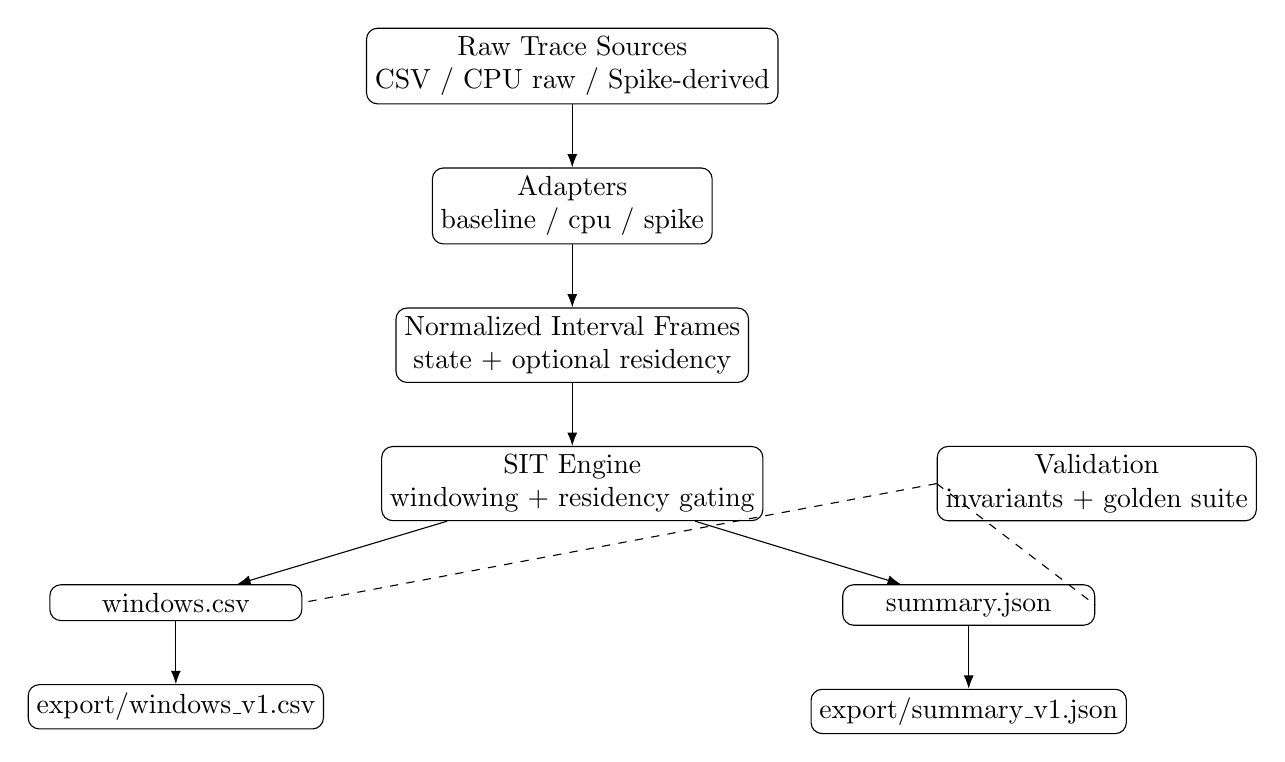
\begin{tikzpicture}[node distance=8mm and 10mm]
    \node[box] (raw) {Raw Trace Sources\\CSV / CPU raw / Spike-derived};
    \node[box, below=of raw] (adp) {Adapters\\baseline / cpu / spike};
    \node[box, below=of adp] (norm) {Normalized Interval Frames\\state + optional residency};
    \node[box, below=of norm] (eng) {SIT Engine\\windowing + residency gating};
    \node[box, below left=of eng] (win) {windows.csv};
    \node[box, below right=of eng] (sum) {summary.json};
    \node[box, below=of win] (expw) {export/windows\_v1.csv};
    \node[box, below=of sum] (exps) {export/summary\_v1.json};
    \node[box, right=22mm of eng] (val) {Validation\\invariants + golden suite};

    \draw[line] (raw) -- (adp);
    \draw[line] (adp) -- (norm);
    \draw[line] (norm) -- (eng);
    \draw[line] (eng) -- (win);
    \draw[line] (eng) -- (sum);
    \draw[line] (win) -- (expw);
    \draw[line] (sum) -- (exps);
    \draw[dashed] (val.west) -- (win.east);
    \draw[dashed] (val.west) -- (sum.east);
  \end{tikzpicture}
  \caption{Phase-1 High-Level Architecture}
\end{figure}

\section{End-to-End Workflow Specification}
\subsection{Pipeline Sequence (TikZ)}
\begin{figure}[H]
  \centering
  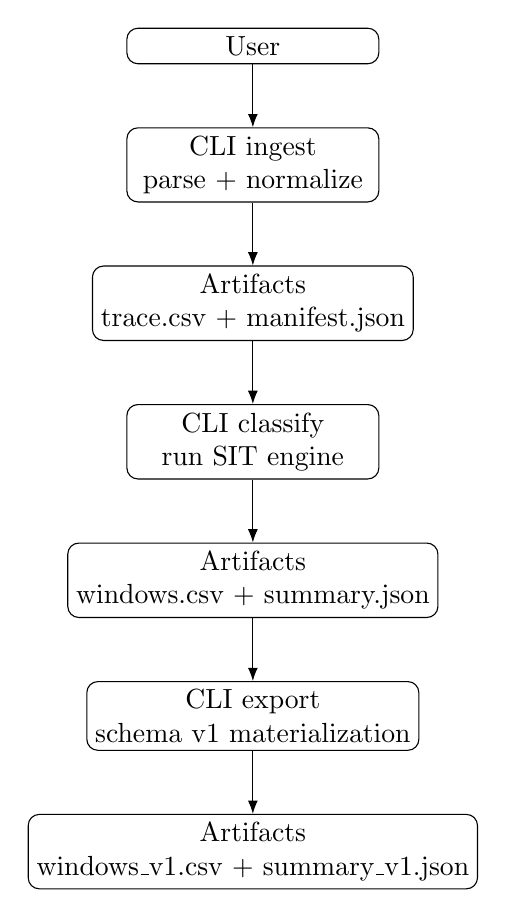
\begin{tikzpicture}[node distance=8mm and 12mm]
    \node[box] (u) {User};
    \node[box, below=of u] (ing) {CLI ingest\\parse + normalize};
    \node[box, below=of ing] (art1) {Artifacts\\trace.csv + manifest.json};
    \node[box, below=of art1] (cls) {CLI classify\\run SIT engine};
    \node[box, below=of cls] (art2) {Artifacts\\windows.csv + summary.json};
    \node[box, below=of art2] (exp) {CLI export\\schema v1 materialization};
    \node[box, below=of exp] (art3) {Artifacts\\windows\_v1.csv + summary\_v1.json};
    \draw[line] (u) -- (ing);
    \draw[line] (ing) -- (art1);
    \draw[line] (art1) -- (cls);
    \draw[line] (cls) -- (art2);
    \draw[line] (art2) -- (exp);
    \draw[line] (exp) -- (art3);
  \end{tikzpicture}
  \caption{End-to-End Workflow}
\end{figure}

\subsection{Workflow Stages}
\begin{longtable}{>{\raggedright\arraybackslash}p{0.20\textwidth} >{\raggedright\arraybackslash}p{0.74\textwidth}}
\toprule
\textbf{Stage} & \textbf{Technical Description} \\
\midrule
Ingest & Reads raw trace source, selects adapter, validates normalized fields, writes \texttt{trace.csv} (+ optional \texttt{residency.csv}), and emits \texttt{manifest.json}. \\
Classify & Executes SIT engine with configured \texttt{window\_us}, computes per-window metrics, and writes \texttt{windows.csv} and \texttt{summary.json}. \\
Export & Applies schema-versioned materialization and writes \texttt{export/windows\_v1.csv} and \texttt{export/summary\_v1.json}. \\
\bottomrule
\end{longtable}

\section{Design Specifications}
\subsection{Adapter Boundary and Normalization}
\begin{itemize}[leftmargin=1.4em]
  \item Engine input is adapter-normalized and source-format agnostic.
  \item State interval contract is strict: \texttt{start\_us}, \texttt{end\_us}, \texttt{core}, \texttt{state}, optional \texttt{work\_done}.
  \item Residency stream is optional and independently normalized.
\end{itemize}

\subsection{Windowing and Boundary Rules}
\begin{figure}[H]
  \centering
  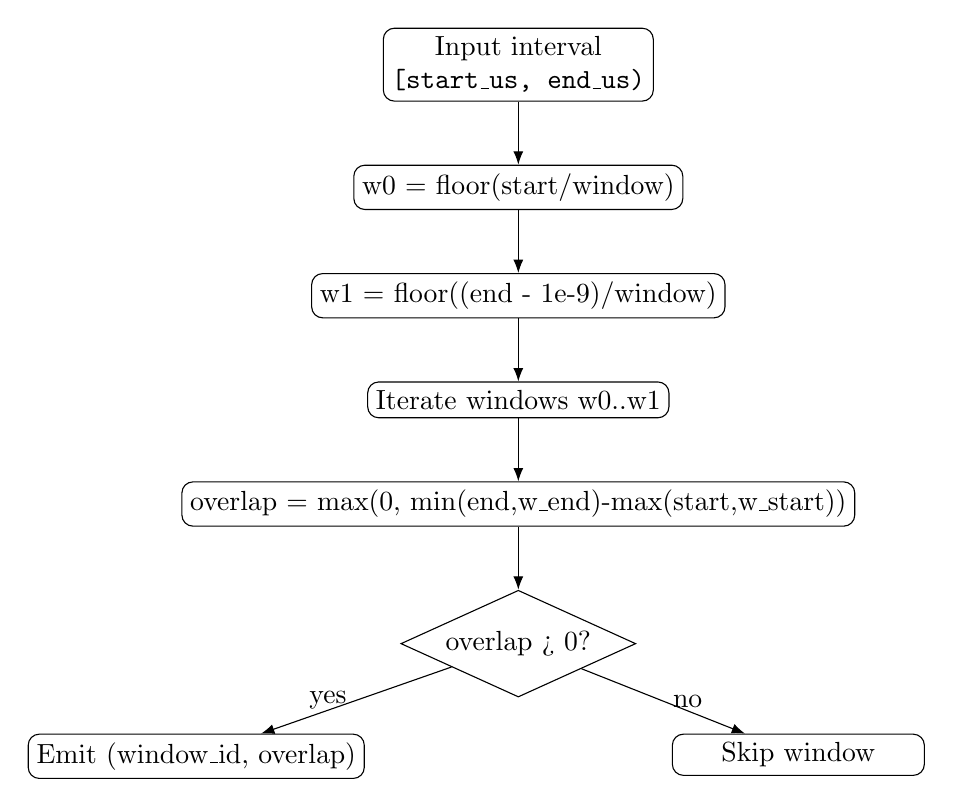
\begin{tikzpicture}[node distance=8mm and 12mm]
    \node[box] (i) {Input interval\\\texttt{[start\_us, end\_us)}};
    \node[box, below=of i] (w0) {w0 = floor(start/window)};
    \node[box, below=of w0] (w1) {w1 = floor((end - 1e-9)/window)};
    \node[box, below=of w1] (iter) {Iterate windows w0..w1};
    \node[box, below=of iter] (ov) {overlap = max(0, min(end,w\_end)-max(start,w\_start))};
    \node[decision, below=of ov] (d) {overlap > 0?};
    \node[box, below left=of d] (emit) {Emit (window\_id, overlap)};
    \node[box, below right=of d] (skip) {Skip window};
    \draw[line] (i) -- (w0);
    \draw[line] (w0) -- (w1);
    \draw[line] (w1) -- (iter);
    \draw[line] (iter) -- (ov);
    \draw[line] (ov) -- (d);
    \draw[line] (d) -- node[left]{yes} (emit);
    \draw[line] (d) -- node[right]{no} (skip);
  \end{tikzpicture}
  \caption{Windowing and Boundary-Exact Overlap Logic}
\end{figure}

\textbf{Boundary rule:} last-window selection uses an epsilon offset on end time to avoid assigning an interval ending exactly on a boundary to the next window.

\subsection{Residency Gating Semantics}
\begin{enumerate}[leftmargin=1.4em]
  \item Merge residency intervals per core.
  \item Intersect state intervals with merged residency mask.
  \item Accumulate active/stall/idle using only intersected durations.
  \item Compute \texttt{resident\_us} independently from residency overlap.
  \item If no residency file is supplied, treat full window duration as resident.
\end{enumerate}

\subsection{Per-Window Metrics}
For each \texttt{(core, window\_id)}:
\begin{itemize}[leftmargin=1.4em]
  \item \texttt{resident\_us}, \texttt{resident\_frac\_of\_window}, \texttt{is\_resident\_window}
  \item \texttt{active\_frac}, \texttt{stall\_frac}, \texttt{idle\_frac}
  \item \texttt{sit}
\end{itemize}

If resident time exists, compute:
\[
\text{sit\_raw} =
\begin{cases}
\frac{\left(\frac{\text{work\_done}}{\text{resident\_us}}\right)}{\text{expected\_work\_rate}} & \text{if work\_done exists} \\
\frac{\text{total\_active\_us}}{\text{total\_resident\_us}} & \text{otherwise (global fallback)}
\end{cases}
\]
\[
\text{sit} = \min(\max(\text{sit\_raw}, 0), 1)
\]

\subsection{Summary Metrics Contract}
Summary statistics are computed across resident windows and include:
\begin{itemize}[leftmargin=1.4em]
  \item \texttt{schema\_version}, \texttt{window\_us}, \texttt{windows\_total}, \texttt{resident\_windows\_total}
  \item \texttt{cores}, \texttt{sit\_median}, \texttt{sit\_p95}
  \item \texttt{residency\_active\_avg}, \texttt{residency\_stall\_avg}, \texttt{residency\_idle\_avg}
  \item \texttt{used\_residency\_file}, \texttt{expected\_work\_rate}
\end{itemize}

\section{Run Directory and Artifact Layout}
\begin{lstlisting}[basicstyle=\ttfamily\small,frame=single]
runs/<run_id>/
  manifest.json
  trace.csv
  residency.csv                # optional
  windows.csv
  summary.json
  export/
    windows_v1.csv
    summary_v1.json
\end{lstlisting}

\section{Validation and QA Specification}
\begin{itemize}[leftmargin=1.4em]
  \item Invariant checks enforce semantic correctness on window outputs.
  \item Golden suite enforces reproducibility across representative datasets.
  \item Phase-0 parity check enforces strict regression on the Wormhole-derived sample trace.
  \item Recommended CI: smoke pipeline $\rightarrow$ invariants $\rightarrow$ golden suite.
\end{itemize}

\subsection{Reference Commands}
\begin{lstlisting}[basicstyle=\ttfamily\small,frame=single]
python cli.py ingest --trace datasets/traces/trace_A_single_residency.csv --out runs/A
python cli.py classify --in runs/A --window-us 256 --residency datasets/residency/partial.csv
python cli.py export --in runs/A --schema v1
python tests/check_invariants.py --windows out/A_partial_windows.csv --mode partial --window-us 256
python tests/run_golden_suite.py --outdir golden_out
python tests/check_phase0_parity.py --windows golden_out/trace_F_phase0_wormhole_sample__base_windows.csv --summary golden_out/trace_F_phase0_wormhole_sample__base_summary.json
\end{lstlisting}

\section{Diagram Rendering Guidance}
This document uses native TikZ diagrams, so no external Mermaid conversion step is required.

\end{document}
